\begin{frame}{Motivation \& Preliminaries}

\only<1,2>{
	\textbf{Proactive-reactive} stochastic project scheduling
	\begin{itemize}
	 	\item stochastic durations $\x{D}=(D_1, \ldots, D_n)$ with known $\mathbb{P}[D_i = t]$
	 	\item solution = (proactive schedule $\x{t}$, reactive policy $\Pi$)
	 	\begin{itemize}
	 		\item $\x{t}=(t_1,\ldots,t_n)$: buffered and can more-or-less be trusted   
	  		\item $\Pi$: what to do in case of buffer overruns
	  	\end{itemize}
	  	\item \textbf{railway mode}: $S_i(\Pi, \x{t}) \geq t_i$
	  	\item find $(\x{t},\Pi)$ that balances \emph{expected instability} and \emph{expected makespan}
	\end{itemize}
	
	\bigskip
	\onslide<2>{
		Minimize both
		\begin{enumerate}
		\item expected instability
		\[
			\mathbb{E}[\sum_{i} (S_i((\Pi,\x{t}),\x{D}) - t_i)]
		\]
		
		\item expected makespan
		\[
			\mathbb{E}[\max_{i} (S_i((\Pi,\x{t}),\x{D}) + D_i)]
		\]
		\end{enumerate}
	}
}

\only<3>{
	Tuning some tradeoff parameter
	\bigskip
	\begin{center}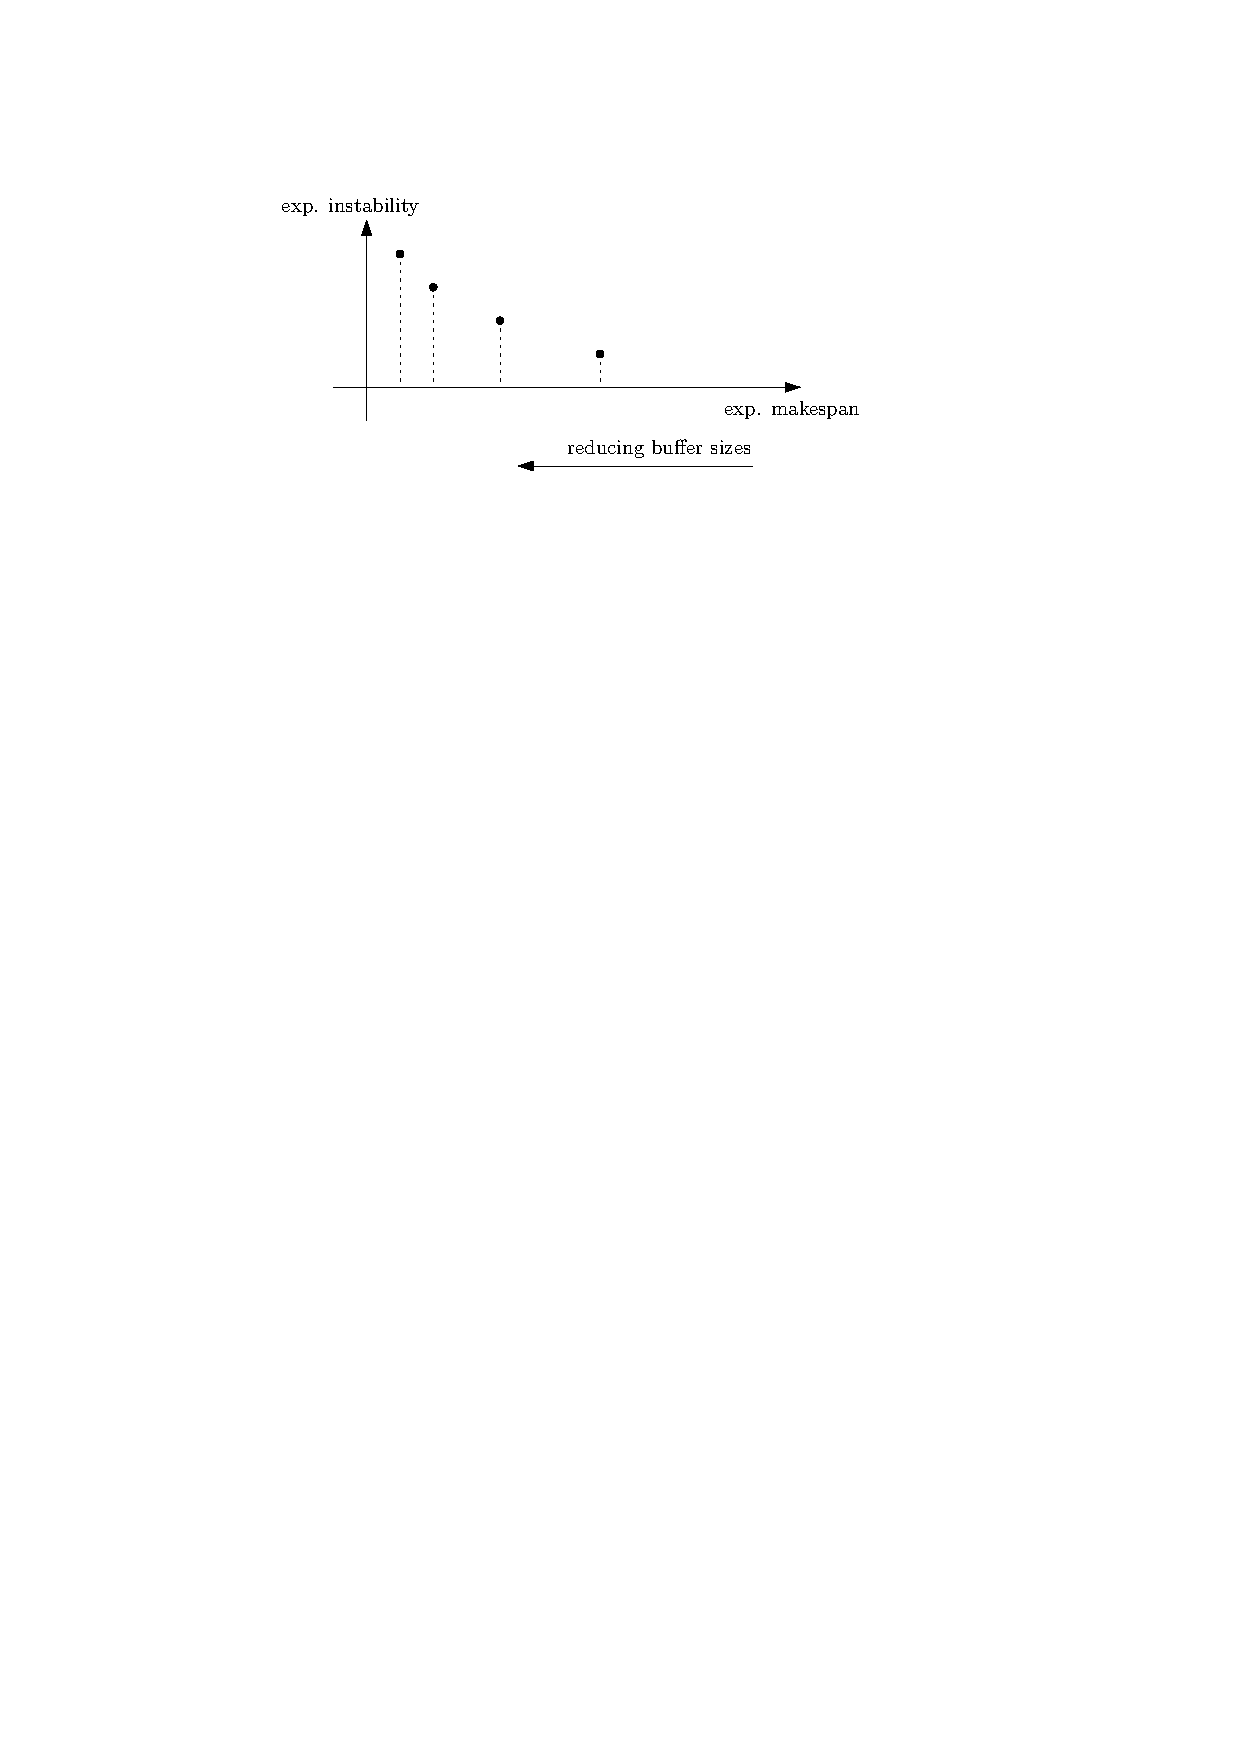
\includegraphics[width=0.7\textwidth]{fig-tradeoff}\end{center}
}

\end{frame}

